\documentclass[11pt, oneside]{article}   	% use "amsart" instead of "article" for AMSLaTeX format
\usepackage{geometry}                		% See geometry.pdf to learn the layout options. There are lots.
\geometry{letterpaper}                   		% ... or a4paper or a5paper or ... 
%\geometry{landscape}                		% Activate for for rotated page geometry
%\usepackage[parfill]{parskip}    		% Activate to begin paragraphs with an empty line rather than an indent
\usepackage{graphicx}				% Use pdf, png, jpg, or eps� with pdflatex; use eps in DVI mode
								% TeX will automatically convert eps --> pdf in pdflatex		
\usepackage{amssymb}
\usepackage{amsmath}
\usepackage{parskip}

\graphicspath{{/Users/telliott_admin/Dropbox/Tex/png/}}

\title{Sums of integers, squared and cubed}
%\author{The Author}
\date{}							% Activate to display a given date or no date

\begin{document}
\maketitle
%\section{}
%\subsection{}
\noindent
\Large
We would like to find formulas for several sums.  To keep it simple, let's start with finite sums like the integers from $1$ to $n$
\[  1 + 2 + 3 + \cdots + n  \]
The numbers we seek are called the triangular numbers.  The triangular numbers are
\[ 1, 3, 6, 10, 15 \cdots \]
Here is a striking "visual proof" of the formula to obtain T$_n$, the $n^{th}$ such number.  The total number of circles in the figure below is $n \times (n+1)$ and this is exactly two times the sum of the integers from $1$ to $n$.
\begin{center} 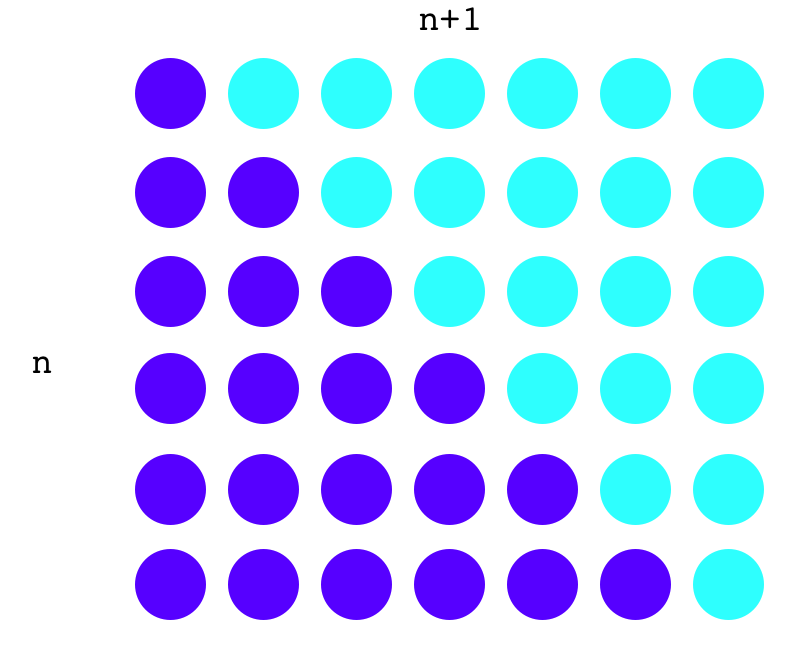
\includegraphics [scale=0.25] {sum_n.png}\end{center}
\[ 2S = n(n+1) \]
There is a famous story about Gauss that, as a schoolboy, he "saw" how to add the integers from $1$ to $100$ as two parallel sums
\[ \ \  1 + \ \ 2 + \ \ 3 + \cdots + 99 + 100 \]
\[ 100 + 99 + 98 + \cdots + 2 + 1 \]
Added together horizontally, these two series must equal twice the sum of $1$ to $100$.  But in the vertical, we notice that we have $n$ sums, each of which is equal to $n+1$.  So, again
\[ 2S = n (n+1) \]
\[ S = \frac{1}{2} \ n (n+1) \]
The value of the sum for $n=100$ is $5050$.  Another way of looking at this result is that between $1$ and $100$ there are $100$ representatives of the "average" value in the sequence, which (because of the monotonic steps) is $(100 + 1)/2 = 50.5$.  Or alternatively, view the sum as ranging from $0$ to $100$ (with the same answer).  Now there are $101$ examples of the average value ($100 + 0)/2 = 50$).

\subsection*{Digression on the method of induction}
\begin{center} 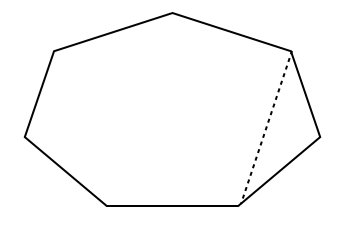
\includegraphics [scale=0.5] {polygon.png} \end{center}
I use my favorite example to introduce the method of induction.  In the figure above we have a polygon---an irregular heptagon.  Actually, there are two polygons, there is the heptagon with $n+1$ sides, and also the hexagon with only $n$ sides that would result from cutting along the dotted line.

What we would like to do is to find a formula for the sum of the internal angles that depends only on the number of sides or vertices.

The first part of the answer is to guess.  In the figure, you can see that by adding the extra vertex to go to the $n+1$-gon, we added a triangle, or perhaps you'd rather say than in going from $n+1$ to $n$ we lost a triangle.  In either case, the difference is $180^\circ$.  The difference between having $n$ sides and $n+1$ sides is to add $180^\circ$.  The second part of the argument is to suppose that $n=3$, in that case we must have simply $180^\circ$ degrees for a triangle.  So we guess that the formula may be
\[ (n-2)180^\circ = S_n \]
where S is the sum of the angles in an $n$-gon.
We can use induction to prove that this formula is correct.

Actually, we've already done the inducing part of induction, when we guessed the formula and verified it for one or a few cases.  Now we'd like to actually prove it.  The proof has two parts.  We must verify the formula for a base case like the triangle, which we've done.  You may wish to check that it works for the square as well, or even a line with two vertices, but that's not necessary.

The second part of the proof is to verify that in going from $n$ to $n+1$, we add another $180^\circ$.  \[ (n-2)180^\circ + 180^\circ \stackrel{?}{=} (n-1)180^\circ \]
On the left-hand side, we have the sum of angles for $n$ sides, which we assume is correct, and then we just add $180^\circ$ to it.  On the right, we have substituted $n+1$ into the formula $((n+1)-2=n-1)$.  Now we need to show that these are equivalent.
But of course
\[ (n-2)x + x = nx - 2x + x = nx + (-2 + 1)x = nx - x = (n-1) x \]
$\square$

That is the inductive proof of the formula.

We can visualize an inductive proof as a kind of chain.  We showed that the "base case" is true, for n = 3.  We also showed that if the formula works for n (when plugging into $n-2(180)=S$), it must work for n+1.

We know it works for $n = 3$;  therefore it works for $n = 4$

We know it works for $n = 4$;  therefore it works for $n = 5$

We know it works for $n = 5$;  therefore it works for $n = 6 \cdots$
\subsection*{Proof of the formula $n(n+1)/2$ by induction}

Returning to the sum of integers, one proof follows the method of induction.  In this approach, however, one must first guess the correct formula.  We guess $n(n+1)/2$, of course.  

Now, we \emph{assume} that the answer is correct for $n$.  We assume:
\[ S_n = \frac{n(n+1)}{2} \]
So clearly, if $S_n$ is correct, then
\[ S_{n+1} = S_n + (n + 1) \]
Follow out the arithmetic:
\[ = \frac{n(n+1)}{2} + \frac{2(n+1)}{2} \]
\[ = \frac{n(n+1) + 2(n+1)}{2} \]
\[ = \frac{(n+1)(n+2)}{2} \]

But this is precisely what we would obtain by using the formula, and substituting $n+1$ for $n$.  Hence the formula gives the correct result for $n+1$, assuming that it gives the correct result for $n$.  In turn, it gives the correct result for $n$, assuming it gives the correct result for $n-1$.  Eventually, we reach the base case, where we can actually verify that the result is correct.

Try it on the first value in the sequence (the "base case").
\[ \frac{1(1+1)}{1} = 1 \]
That checks.  So the whole chain of reasoning is correct.  $\checkmark$

\subsection*{Derivation using sums}
It seems a shame to spoil such a beautiful proof "without words" as the one above by saying anything more, but I can't resist.  I'd like to derive the equation we have been using using algebra.  The general method will help us later.

For any number $k$ it is true that
\[ (k+1)^2 = k^2 + 2k + 1 \]
So consider what happens if we sum the values from $k=1 \rightarrow n$ for each of these terms
\[ \sum_{k=1}^n (k+1)^2 = \sum_{k=1}^n k^2 + \sum_{k=1}^n 2k + \sum_{k=1}^n 1 \]
If the sum is valid for any individual $k$, then it is also true plugging in all $k$ up to $n$.

Rearranging
\[ \sum_{k=1}^n (k+1)^2 - \sum_{k=1}^n k^2 = \sum_{k=1}^n 2k + \sum_{k=1}^n 1 \]
Now think about the left-hand side in our equation. 
\[ \sum_{k=1}^n (k+1)^2 - \sum_{k=1}^n k^2 \]
If we count down rather than up, start with $k=n$.  We have the following terms
\[ k = n \rightarrow \ \ (n+1)^2 - (n)^2 \]
\[ k = n-1 \rightarrow \ \ (n)^2 - (n-1)^2 \]
\[ k = n-2 \rightarrow \ \ (n-1)^2 - (n-2)^2 \]
\[ \cdots \]
\[ k = 1 \rightarrow \ \ (2)^2 - (1)^2 \]

Adding everything together, we obtain
\[ S = (n+1)^2 - (n)^2 + (n)^2 - (n-1)^2 + (n-1)^2 - (n-2)^2 + \cdots + (2)^2 - (1)^2 \]

Notice how all the terms except the first and last cancel.  This is called a "collapsing" or "telescoping" sum.  We have
\[ S = (n+1)^2 - 1 \]
\[ = n^2 + 2n \]

Bringing back the right-hand side  we have
\[ n^2 + 2n = \sum_{k=1}^n 2k + \sum_{k=1}^n 1 \]
We can bring the constant factor $2$ out of the sum, and also, we recognize that the sum of the value $1$ a total of $n$ times is just $n$.
\[ n^2 + 2n = 2\sum_{k=1}^n k + n \]

Subtract $n$ from both sides and divide by $2$:
\[ \sum_{k=1}^n k = \frac{n (n+1)}{2} \]
That's it!

\subsection*{Sum of Squares}
\begin{center} 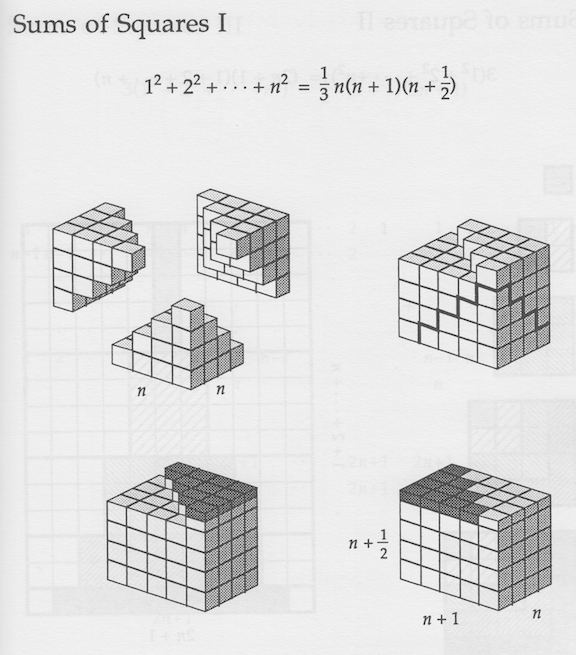
\includegraphics [scale=0.5] {sum_n2.png}\end{center}
Our next sum is that of the squares of the first $n$ integers.  There is a visual proof for this one as well (above).
\[ \sum_{k=1}^n k^2 \]
We obtain (by methods we will see below) the formula
\[ \sum_{k=1}^n k^2 = \frac{n(n+1)}{2} \frac{2n+1}{3} \]
\[ = \frac{n(n+1)(2n+1)}{6} \]
This formula is also written as
\[  \sum_{k=1}^n k^2 = \frac{1}{6} \ (2n^3 + 3n^2 + 2n) \]
\[ = \frac{n^3}{3} + \frac{n^2}{2} + \frac{n}{3} \]
We can check it by induction.  The base case is easy
\[ \frac{1(2)(3)}{6} = 1 \]  
$\checkmark$  

Now for the induction step:
\[ \frac{n(n+1)(2n+1)}{6} + (n+1)^2 \]
\[ = \frac{n+1}{6}  \ [ \ (n)(2n+1) + 6(n+1) \ ] \]
Look at what's in the brackets
\[ (n)(2n+1) + 6(n+1) \]
\[ = 2n^2 + 7n + 6 \]
\[ = (n + 2)(2n + 3) \]
\[ = (n + 1 + 1)(2(n + 1) + 1) \]
So altogether we have
\[ = \frac{(n+1)(n + 1 + 1)(2(n + 1) + 1)}{6} \]
which indeed, is the formula we had above, substituting $n+1$ for $n$.

\subsection*{Strang's proof}
Here are two more approaches.  The first one is in Strang's \emph{Calculus}.  He says "the best place to start is a good guess".  So again, our goal is to find a formula for:

\[ S = \sum_{k=1}^{n} \ k^2 \]

Perhaps we visualize a pile of cannonballs

\begin{center} 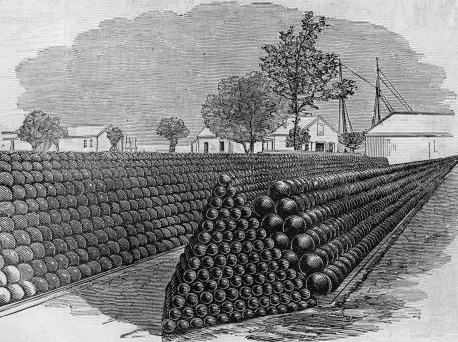
\includegraphics [scale=0.5] {cannonballs.png} \end{center}


Each layer contains a square number of cannonballs ($1$, then $4$, then $9$, etc.).  The shape is a pyramid with dimensions $n \times n \times n$.  We know the formula for the volume of a pyramid, and guess

\[ S_n = \frac{1}{3} n^3 \]

To test it, check whether this difference is $n^2$ (as it should be):

\[ S_{n} - S_{n-1} = \frac{1}{3} n^3 - \frac{1}{3} (n-1)^3 \]

Now

\[ (n-1)^2 = n^2 - 2n + 1 \]
\[ (n-1)^3 = (n-1)(n^2 - 2n + 1) \]
\[ = n^3 - 3 n^2 + 3 n - 1\]

So

\[ S_{n} - S_{n-1} = \frac{1}{3} (n^3 - n^3 + 3 n^2 - 3 n + 1) \]

We see that our guess is off by the residual terms

\[ \frac{1}{3} (3 n^2 - 3 n + 1) \]
\[ = n^2 - n + \frac{1}{3} \] 

Strang says:  the guess needs \emph{correction terms}.  
To cancel $1/3$ in the difference, subtract $n/3$ from the sum.  And to add back $n$ in the difference, add back $1 + 2 + \dots + n(n+1)/2$ to the sum.  Our new guess is

\[ S_n =  \frac{1}{3} n^3 + \frac{n(n+1)}{2} - \frac{n}{3} \]
\[ = \frac{n}{6} (2n^2 + 3(n+1) - 2) \]
\[ =  \frac{n}{6} (2n + 1)(n + 1) \]
\[ = \frac{n(n+1)(2n+1)}{6} \]

which may be easier to remember as

\[ S_n = \frac{n(n+1)}{2} \times \frac{2n + 1}{3} \]

\subsection*{Derivation by collapsing sum}

We proceed as we did in the case of the sum of integers.  There we used $(k+1)^2$ and worked out the consequences.  Here we use

\[ (k+1)^3 = k^3 + 3k^2 + 3k + 1 \]

We sum everything.

\[ \sum_{k=1}^n (k+1)^3 = \sum_{k=1}^n k^3 + \sum_{k=1}^n 3k^2 + \sum_{k=1}^n 3k + \sum_{k=1}^n 1 \]

As before, subtract the first term on the right from the left-hand side, giving us a collapsing sum.  We obtain

\[ \sum_{k=1}^n (k+1)^3 - \sum_{k=1}^n k^3 = (n+1)^3 - 1 \]
\[ = n^3 + 3n^2 + 3n \]

Recognize that the last sum is just $n$ 

\[ \sum_{k=1}^n 1 = n \]

subtract it from $3n$

\[ = n^3 + 3n^2 + 2n \]
\[ = n(n^2 + 3n + 2) \]
\[ = n(n+1)(n+2) \]

Assembling everything

\[ n(n+1)(n+2) = \sum_{k=1}^n 3k^2 + \sum_{k=1}^n 3k \]

We pull out the factor of $3$ from the sums

\[ n(n+1)(n+2) = 3\sum_{k=1}^n k^2 + 3\sum_{k=1}^n k  \]

The first sum on the right is what we seek, the second one is what we obtained before

\[ n(n+1)(n+2) = 3\sum_{k=1}^n k^2 + \frac{3}{2}\ n(n+1) \]

Multiply by $2$

\[ 2n(n+1)(n+2) = 6\sum_{k=1}^n k^2 + 3n(n+1) \]

Rearrange

\[ 6\sum_{k=1}^n k^2 = 2n(n+1)(n+2) - 3n(n+1) \]

Factor out the $n(n+1)$

\[ 6\sum_{k=1}^n k^2 = n(n+1) \ [ \ 2(n + 2) - 3 \ ] \]
\[ 6\sum_{k=1}^n k^2 = n(n+1)(2n + 1) \]
\[ \sum_{k=1}^n k^2 = \frac{n(n+1)}{2} \ \frac{(2n + 1)}{3}  \]

\subsection*{Sum of Cubes}

Let's do one more.  It will help in working out the Riemann Sum for $n^3$.  We proceed exactly as before

\[ (k+1)^4 = k^4 + 4k^3 + 6k^2 + 4k + 1 \]

Sum each term from $k=1 \rightarrow k=n$

\[ \sum_{k=1}^n (k+1)^4 = \sum_{k=1}^n k^4 + \sum_{k=1}^n 4k^3 + \sum_{k=1}^n 6k^2 + \sum_{k=1}^n 4k + \sum_{k=1}^n 1 \]

Rearrange and compute the collapsing sum.

\[ \sum_{k=1}^n (k+1)^4 - \sum_{k=1}^n k^4 = \sum_{k=1}^n 4k^3 + \sum_{k=1}^n 6k^2 + \sum_{k=1}^n 4k + \sum_{k=1}^n 1 \]

\[ (n+1)^4 - 1 = \sum_{k=1}^n 4k^3 + \sum_{k=1}^n 6k^2 + \sum_{k=1}^n 4k + \sum_{k=1}^n 1 \]

Substitute for the right-hand sum

\[ (n+1)^4 - 1 = \sum_{k=1}^n 4k^3 + \sum_{k=1}^n 6k^2 + \sum_{k=1}^n 4k + n \]

Rearrange some more

\[ \sum_{k=1}^n 4k^3 = (n+1)^4 - 1 - \sum_{k=1}^n 6k^2 - \sum_{k=1}^n 4k - n \]

Expand the term $(n+1)^4$ and pick up the $-1 - n$:

\[ (n+1)^4 - 1 - n \]
\[ = n^4 + 4n^3 + 6n^2 + 4n + 1 - 1 - n \]
\[ =  n^4 + 4n^3 + 6n^2 + 3n  \]

Factor out an $n$

\[ = (n)(n^3 + 4n^2 + 6n + 3) \]

And another $n+1$

\[ = (n)(n+1)(n^2 + 3n + 3) \]

Recall our previous results:

\[ \sum_{k=1}^n 6k^2 = 6 \sum_{k=1}^n k^2 \]
\[ = 6 \ \frac{n(n+1)(2n+1)}{6}  \] 
\[ = n(n+1)(2n+1) \] 

Similarly

\[ \sum_{k=1}^n 4k = 4 \sum_{k=1}^n k \]
\[ = 4 \ \frac{n(n+1)}{2} \]
\[ = 2 n(n+1) \]

Substitute all three of these results (and pull out the factor of $4$ from the sum):

\[ 4\sum_{k=1}^n k^3 = (n)(n+1)(n^2 + 3n + 3) - n(n+1)(2n+1) -  2 n(n+1) \] 

Just a bit more algebra.  See that we have $n(n+1)$ in each term.  We have

\[ = n(n+1) \ [ \ (n^2 + 3n + 3) - (2n+1) -  2 \ ]  \]
\[ = n(n+1) \ [ \ n^2 + 3n + 3 - 2n - 1 -  2 \ ]  \]
\[ = n(n+1) \ [ \ n^2 + n  \ ]  \]
\[ = n(n+1)  \cdot  n(n+1)  \]

So all together we have

\[ 4\sum_{k=1}^n k^3 = n(n+1) \cdot n (n+1) \] 
\[ \sum_{k=1}^n k^3 = \frac{n(n+1)}{2} \cdot \frac{n (n+1)}{2} \] 
\[ \sum_{k=1}^n k^3 = \ [ \ \frac{n(n+1)}{2} \ ]^2 \] 

A remarkable simplification!

I have some other write-up about these problems, which I appended below.  But we could just look at another beautiful proof without words

\begin{center} 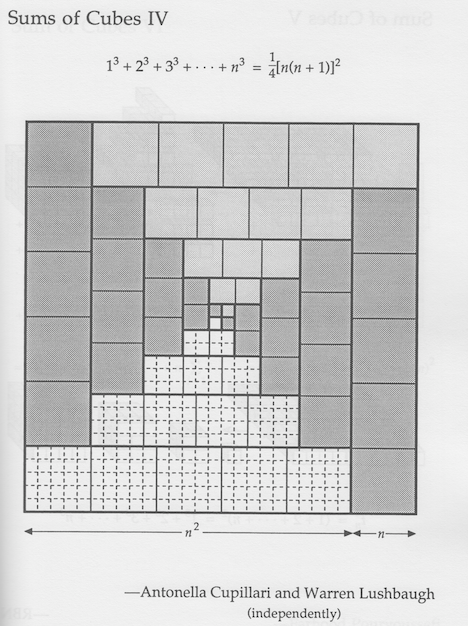
\includegraphics [scale=0.75] {sum_n3.png}\end{center}

\subsection*{Analysis}

We have shown in other write-ups, and you can easily verify by searching that the sum of the integers between $1$ and $n$ is 
\[ 1 + 2 + \dots + n = \sum\limits_{k=1}^n k = \frac{n(n+1)}{2} \]
The next one, the sum of the squares of the first $n$ integers, is useful for certain derivations in calculus (e.g. the Riemann sum to integrate $y=x^2$)
\[ 1^2 + 2^2 + \dots + n^2 = \sum\limits_{k=1}^n k^2 = \frac{n(n+1)(2n+1)}{6} \]
\[ = \frac{n^3}{3} + \frac{n^2}{2} + \frac{n}{3} \]
I was quite surprised to find that the sum of cubes is also simple and frankly, amazing
\[ 1^3 + 2^3 + \dots + n^3 = \sum\limits_{k=1}^n k^3 = \frac{n^2(n+1)^2}{2^2} = [\ \frac{n(n+1)}{2}\ ]^2 = [\ \sum\limits_{k=1}^n k \ ] ^2 \]
\begin{equation}
\boxed{ \sum\limits_{k=1}^n k^3 = [\ \sum\limits_{k=1}^n k \ ] ^2}
\end{equation}
Let's just try to prove the last formula using induction.

The "base case" is pretty simple.  For $n=2$
\[ 1^3 + 2^3 = 1 + 8 = 9 \]
and
\[ \frac{n^2(n+1)^2}{2^2} = \frac{2^2(3^2)}{2^2} = 3^2 = 9 \]
Check.  Now for the induction step what we need to show is that what we get assuming the formula for $n$ is correct and then adding the term $(n+1)^3$
\begin{equation}
\boxed{ \frac{n^2(n+1)^2}{2^2} + (n+1)^3}
\end{equation}
is equal to what we get by plugging $n+1$ into the formula.
\begin{equation}
\boxed{ \frac{(n+1)^2(n+2)^2}{2^2}}
\end{equation}
We need to show that eqn 2 is equal to eqn 3.  
\[ \frac{n^2(n+1)^2}{2^2} + (n+1)^3 = \frac{(n+1)^2(n+2)^2}{2^2} \]
First, we can factor out and cancel $(n+1)^2$ from both sides.  So then we have
\[ \frac{n^2}{2^2} + (n+1) \stackrel{?}{=} \frac{(n+2)^2}{2^2} \]
\[ n^2 + 4(n+1) \stackrel{?}{=} (n+2)^2 \]
Sure, that looks correct!  And we're done with the proof by induction, so we can put a little box.

$\square$

\subsection*{Looking deeper}
\[ \sum\limits_{k=1}^n k^3 = [\ \sum\limits_{k=1}^n k \ ] ^2 \]
I wanted to try to understand something more about why this is true.  A simple web search revealed the answer.  Here's an interesting pattern for the cubes of integers that I'd never seen before
\[ 1^3 = 1 \]
\[ 2^3 = 8 = 3 + 5 \]
\[ 3^3 = 27 = 7 + 9 + 11 \]
\[ 4^3 = 64 = 13 + 15 + 17 + 19 \]
\[ 5^3 = 125 = 21 + 23 + 25 + 27 + 29  \]

If you want a formula for $n^3$, notice that the first term is $n^2 - n + 1$ and the last term is $n^2 - n + 2n - 1$, and the number of terms for each sum equals $n$.  (There are $n$ odd numbers between $1$ and $2n-1$).

In other words, the sum of all the cubes of integers from $1^3$ to $n^3$ is equal to the sum of all the odd numbers up to $n^2 - n + 2n - 1 = n^2 + n - 1$.

How many of these numbers are there?  A little thought should convince you that the answer is $(n^2 + n)/2$.  For example, with $n=5$, our last odd number is $5^2 + 5 - 1 = 29$, and we have $(25 + 5)/2 = 15$ terms.

We want the sum of the first $(n^2 + n)/2$ odd numbers.

Let's look at another pattern
\[ 1 = 1 \]
\[ 2^2 = 4 = 1 + 3 \]
\[ 3^2 = 9 = 1 + 3 + 5 \]
\[ 4^2 = 16 = 1 + 3 + 5 + 7 \]
\[ 5^2 = 25 = 1 + 3 + 5 + 7 + 9 \]

The \emph{odd number theorem} says that the sum of the first $n$ odd numbers is equal to $n^2$.  We want the sum of the first $(n^2 + n)/2$ odd numbers, so that's $((n^2 + n)/2)^2$.  And that's how we get our formula.

\end{document}  